% !Mode:: "TeX:UTF-8"
%% 请使用 XeLaTeX 编译本文.
% \documentclass{WHUBachelor}% 选项 forprint: 交付打印时添加, 避免彩色链接字迹打印偏淡. 即使用下一行:
 \documentclass[forprint]{WHUBachelor}
\usepackage{cite} 
\usepackage{amsmath, amsfonts, amssymb} % math equations, symbols
\usepackage[english]{babel}
\usepackage{color}      % color content
\usepackage{graphicx}   % import figures
\usepackage{url}        % hyperlinks
\usepackage{bm}         % bold type for equations
\usepackage{multirow}
\usepackage{booktabs}
\usepackage{epstopdf}
\usepackage{epsfig}
\usepackage{algorithm}
\usepackage{algorithmic}
\usepackage{esvect}
\usepackage{listings}
\usepackage[framed,numbered,autolinebreaks,useliterate]{mcode}
\usepackage{subfig}
\usepackage{float}
\begin{document}
%%%%%%% 下面的内容, 据实填空.


\StudentNumber{力6} % 填写自己的学号

\title{\\有限元法基础\\桥梁设计竞赛报告}

\advisor{张雄教授}

\author{毕恺峰$\,$ 胡昌平$\,$ 黄轩宇 $\,$易泽吉$\,$张逸葑}                            % 作者名字

\Cmajor{工程力学}                  % 专业中文名

\Cschoolname{航天航空学院}          % 学院名

\date{二〇一八年三月}                    % 日期, 要注意和英文日期一致!!


%-----------------------------------------------------------------------------
\pdfbookmark[0]{封面}{title}         % 封面页加到 pdf 书签
\maketitle
\frontmatter
\pagenumbering{Roman}              % 正文之前的页码用大写罗马字母编号.
%-----------------------------------------------------------------------------

%==========================把目录加入到书签==============================%%%%%%
\pdfbookmark[0]{目录}{toc}

\mainmatter %% 以下是正文、
\tableofcontents
\chapter{摘要}
\chapter{桥梁的基本选择与设计思路}
\section{悬索斜拉桥}
\section{拱形桥}
\section{xx桥}
\section{xx桥}
\chapter{桥梁的Abaqus实现}
\section{零件的设计}
\section{有限元单元类型的选择}
\section{有限元单元尺寸的选择}
\section{施加约束条件}

\chapter{桥梁的cost计算}

\section{Abaqus-Python脚本读取过程}
在桥梁的大体结构设计确定之后,在进行几何参数改良时,如果在CAE界面改参数将变得非常繁琐,而将模型进行python录制后直接读入相关参数进行计算将非常方便;与此同时,由于我们最终需要集中优化的参数为桥梁的最大位移,桥梁的总造价和承载应力情况,而CAE界面只能查看应力的大体分布情况,无法对所有单元的应力分布情况做一个具体的分析,因此我们还需要利用python脚本对整个Abaqus数据结构进行有选择性的数据读取,其中主要包括节点位移,单元应力,以及单元对应的高斯点坐标,单元几何属性等;与此同时我们可以利用matlab等软件作为python的外部接口,即为python脚本提供输入数据(inp文件),并对输出数据进行相应的分析。整个脚本的程序逻辑结构如图\ref{4-1}所示:

\begin{figure}[H]
\centering  
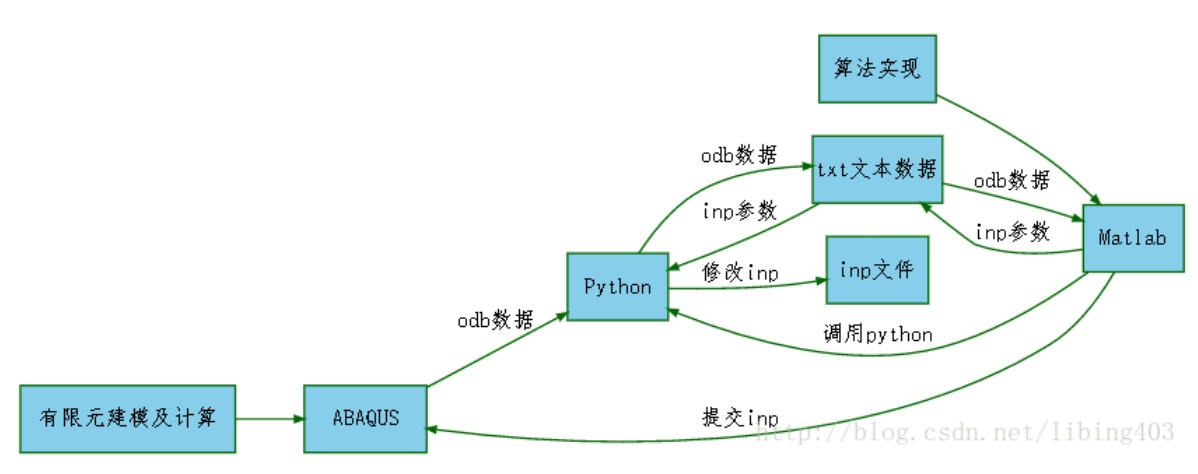
\includegraphics[width = .8\textwidth]{1.png} 
\caption{python后处理设计逻辑} 
\label{4-1} 
\end{figure}

\subsection{ODB对象数据结构:}

如图\ref{4-2}所示:ODB对象主要对包含计算模型对象数据(Model Data)和计算结果数据(Result Data),计算模型对象数据包含装配体(rootAssenbly)
、零件(parts) 、界面分类(sectionCategories)、材料(materials) 等子对象,计算结果数据steps包含分析步(step)
、帧(frame) 、历史变量输出(historyoutputs) 和场变量输出(field outputs) 等。场变量的读取路径:odb.Setps{[}{]}.frames{[}{]}.fieldOutputs{[}{]};

场变量包括:应力分量-'S';应-'E'; 位移-'U';

历史变量的读取路径:odb.Setps{[}{]}.historyRegions{[}{]}.historyOutputs{[}{]};

\begin{figure}[H]
\centering  
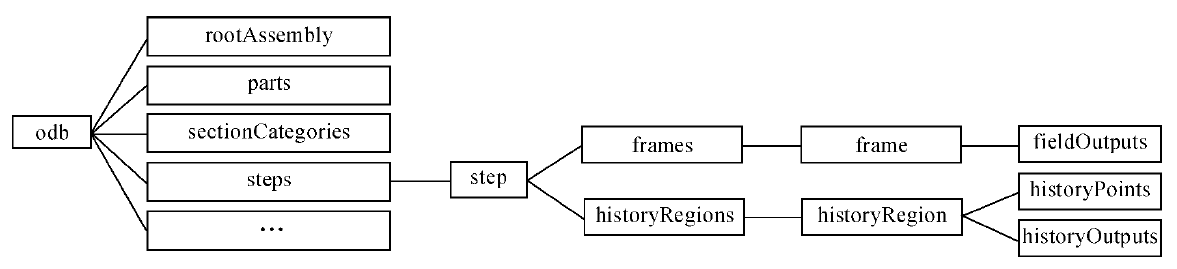
\includegraphics[width = .8\textwidth]{2.png} 
\caption{Abaque odb数据结构示意图} 
\label{4-2} 
\end{figure}

\subsection{MDB对象数据结构}

如图\ref{4-3}所示:MDB对象主要对包含计算模型对象数据(Model Data) 和工作对象数据(Job Data) ,其中model对象,包含零件(parts)
、材料(materials) 等子对象。零件(parts) 子对象包含单元(elements) 、集合(sets) 和节点(nodes)
子对象,其下又包含编号(label) 、坐标(coordinate) 、单元所属节点组(connectivity)等属性。

几何集的读取路径:mdb.models{[}{]}.parts{[}{]}.sets{[}{]}.odb.rootAssembly.instance{[}{]}.elementSets{[}{]};

几何集所属单元,节点信息读取路径:

单元编号:mdb.models{[}{]}.parts{[}{]}.sets{[}{]}.elements{[}{]}.elementLabel.odb.rootAssembly.Instances{[}{]}.elementSets{[}{]}.elements{[}{]}.
elementLabel;

单元所属节点组:mdb.models{[}{]}.parts{[}{]}.sets{[}{]}.elements{[}{]}.Connectivity.odb.
rootAssembly.instances{[}{]}.elementSets{[}{]}. elements{[}{]}. connectivity;

节点坐标:mdb.models{[}{]}.parts{[}{]}.sets{[}{]}.nodes{[}{]}.coordinates;

\begin{figure}[H]
\centering  
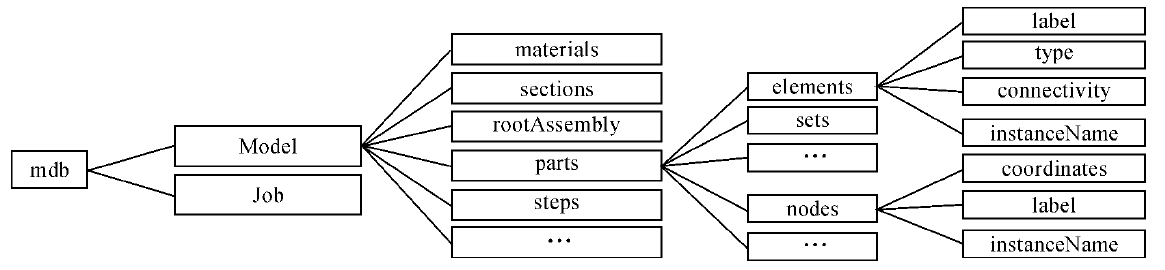
\includegraphics[width = .8\textwidth]{3.png} 
\caption{Abaque mdb数据结构示意图} 
\label{4-3} 
\end{figure}

\subsection{最大位移读取}

我们在odb对象中把位移场’U’的数据读取出来,然后对节点进行循环得到最大的位移数值,如图\ref{4-4}所示:

\begin{figure}[H]
\centering  
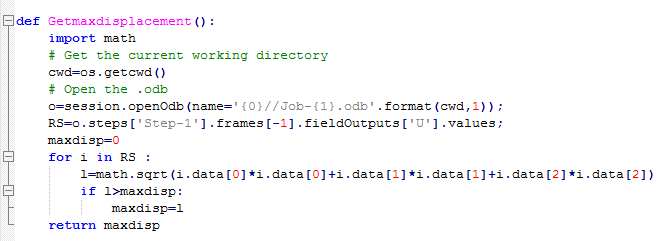
\includegraphics[width = .8\textwidth]{4.png} 
\caption{最大位移读取程序示意图} 
\label{4-4} 
\end{figure}

\subsection{单元应力和最大许用应力}

首先先在odb对象中把应力场’S’中的数据读取出来,然后再将其写入txt文件中,同时输入相应的单元类型和单元号,以便之后对应相应的单元属性,如图\ref{4-5}所示:

\begin{figure}[H]
\centering  
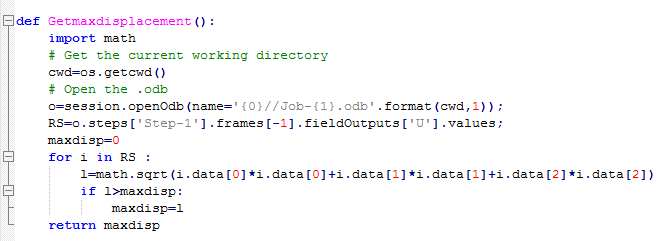
\includegraphics[width = .8\textwidth]{4.png} 
\caption{应力读取程序示意图} 
\label{4-5} 
\end{figure}

\subsection{单元属性读取}

最后我们在mdb对象中得到所有单元的材料属性和坐标等参数,写入到另一个txt文件中,如图\ref{4-6}所示:

\begin{figure}[H]
\centering  
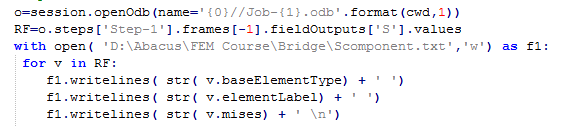
\includegraphics[width = .8\textwidth]{5.png} 
\caption{单元属性读取程序示意图} 
\label{4-6} 
\end{figure}

之后再将相关的单元应力和单元信息参数一同导入到matlab中进行相关的循环检索,利用超过许用应力的单元对应到其单元类型,利用其单元数据计算出其体积;最后检索所有的单元信息得到所有单元的体积总和,一方面计算相应的参数


\chapter{桥梁的优化过程}
\section{算法的选择}
\section{程序设计思路}
\section{优化实例}
\chapter{优化服务器}
\section{Abaqus的GPU优化构架}
\section{服务器的CPU-GPU取舍}
\chapter{结论}
最终我们选取的桥梁如下。。。Abaqus相关文件见。。。。总体的cost为。。。。
\bibliographystyle{plain}
\bibliography{bridge_report}
\cleardoublepage
\end{document}

%%%============================================================================================================%%%

%%%=== 参考文献 ========%%%




